%\VignetteEngine{knitr::knitr}
%\VignetteIndexEntry{Starting with bipartite}
%\VignetteEncoding{UTF-8}

\documentclass[a4paper, 11pt]{article}\usepackage[]{graphicx}\usepackage[]{color}
%% maxwidth is the original width if it is less than linewidth
%% otherwise use linewidth (to make sure the graphics do not exceed the margin)
\makeatletter
\def\maxwidth{ %
  \ifdim\Gin@nat@width>\linewidth
    \linewidth
  \else
    \Gin@nat@width
  \fi
}
\makeatother

\usepackage{Sweavel}


%\usepackage[sc]{mathpazo}
%\usepackage{authblk} % authors & affiliations
\usepackage[utf8]{inputenc}
\usepackage{geometry}
  \geometry{verbose,tmargin=2cm,bmargin=2cm,lmargin=3cm,rmargin=2cm}
  \setcounter{secnumdepth}{3}
  \setcounter{tocdepth}{3}
%\setlength{\parskip}{\bigskipamount}
%\setlength{\parindent}{0pt}
\usepackage{makeidx}
  \makeindex
\usepackage{natbib}
\usepackage{url}
\usepackage[unicode=true,pdfusetitle,
 bookmarks=true,bookmarksnumbered=true,bookmarksopen=true,bookmarksopenlevel=2,
 breaklinks=true,pdfborder={0 0 1},backref=true,colorlinks=false, hidelinks]
 {hyperref}
%\hypersetup{ pdfstartview={XYZ null null 1}}
\usepackage{breakurl}
\usepackage{titlesec} % for titleformat
\usepackage[nottoc]{tocbibind} % include reference in table of content
\usepackage{wrapfig}
\usepackage[dvipsnames]{xcolor}

%\makeatletter
%%%%%%%%%%%%%%%%%%%%%%%%%%%%%% User specified LaTeX commands.
% % % % % % %  section numbering onto margins % % % %
\newlength\mylensection
\setlength\mylensection{\dimexpr\oddsidemargin+1cm+\hoffset\relax}
\titleformat{\section}{\normalfont\Large\itshape}{\llap{\hspace*{-\mylensection}\textcolor{YellowGreen}{\textbf{\LARGE{ \thesection}}}\hfill}}{0em}{} %

\newlength\mylensubsection
\setlength\mylensubsection{\dimexpr\oddsidemargin+1cm+\hoffset\relax}
\titleformat{\subsection}{\normalfont\large\itshape}{\llap{\hspace*{-\mylensubsection}\textcolor{YellowGreen}{\textbf{\Large{ \thesubsection}}}\hfill}}{0em}{} %


\renewcommand{\textfraction}{0.05}
\renewcommand{\topfraction}{0.8}
\renewcommand{\bottomfraction}{0.8}
\renewcommand{\floatpagefraction}{0.75}

\newcommand{\package}[1]{\textbf{#1}}
\newcommand{\proglang}[1]{\textsl{#1}}
\newcommand{\code}[1]{\texttt{#1}}
\newcommand{\ind}[1]{#1\index{#1}}           			   % \ind{bla} instead of bla\index{bla}
\newcommand{\indE}[1]{\emph{#1}\index{#1@\emph{#1}}}       % dito for emphasised words (e.g. English)
\newcommand{\indR}[1]{\texttt{#1}\index{#1@\texttt{#1}}}   % dito for typewriter


\renewcommand{\vec}[1]{\mathbf{#1}}                   % replaces the arrow over vectors by bold-print


%\makeatother
\frenchspacing % avoid long spaces after a "."

\begin{document}


\title{Using bipartite to describe and plot two-mode networks in \proglang{R}}

\author{Carsten F. Dormann\\Biometry \& Environmental System Analysis\\University of Freiburg, Germany
\and Jochen Fründ\\Biometry \& Environmental System Analysis\\University of Freiburg, Germany}

%\thanks{\href{mailto:carsten.dormann@biom.uni-freiburg.de}{carsten.dormann@biom.uni-freiburg.de}}

\maketitle

\begin{abstract}
\noindent This vignette introduces the bipartite package to newbees. It describes it intention and, in seperate sections, the use of the most important functions.
\end{abstract}

\tableofcontents


\section{Introduction}
\subsection{Introduction for ecologists}
Many interactions between species are between distinct groups, such as pollinators and flowers, or herbivores and plants, or parasitoids and their hosts, or predators and their prey. When no information on interactions \emph{within} groups is known, we have the case of a \emph{bipartite} (a.k.a. ``two-mode'') network. In constrast, if every species could interact with every other, and we have (necessarily incomplete) information on these interactions, we have the case of a ``unipartite'' or ``one-mode'' network (think: food web). 

\subsection{Introduction for non-ecologists}
In mathematics, there is a field called ``graph theory'', which describes/analyses/formalises ``graphs'' and the operations among them. A graph consists of \emph{nodes} and \emph{edges} (which are the links between nodes). A node can be something like an airport with edges being the flights between them; a power grid of power plants and energy consumers, with the power lines being the edges; a list of industry ``leaders'' and the edges representing financial ties between them; or, e.g. in ecology, a list of species, with edges representing trophic relationships, i.e. who eats whom.

When the nodes are grouped into two distinct sets, with no (known or quantified) interactions \emph{within} a set, then we call it a bipartite network (``two parts'', a.k.a. ``two-mode'' network). In our examples these could be airports of different continents (and no intracontinental flights are in our data base); power plants and energy consumers; industry executives and companies (where an executive can sit in the board of different companies); or pollinators and plants.

\subsection{Introduction continued for both, ecologists and non-ecologists}
This vignette tries to illustrate and explain a package that deals almost exclusively with \emph{bipartite} networks!

The typical tasks we want to carry out are
\begin{enumerate}
\item visualise the network;
\item compute network indices to summarise its structure;
\item statistically test for differences between networks;
\item statistically test for differences between observed and random networks.
\end{enumerate}
\package{bipartite} aims to facilitate this steps. This vignette aims to facilitate the use of \package{bipartite}. We shall try to predominantly use the technical terms (``node'' and ``edges''), but our examples will be from the ecological realm, where nodes are (typcially) species, and edges are typically called ``links'', which in fact are observed (or assumed) ecological interactions (such as pollination, predation, dispersal). Apologies for mixing these two!

Also, as ecologists we are not ``graph theoreticians'' or mathematicians. Often, in the ecological literature, mathematical terms are used to elevate the status of the author, at no benefit to the analysis or to the reader. We are hesitant to use pretend-mathematics, at the risk of sounding daft to a person familiar with graph theory.

Of course, we don't mind if this documented would be cited, e.g. as \citet{bipartiteVignette}. Alternatively, you can always cite our work on this subject, inevitably also using (some functionality of) \package{bipartite} \citep{Dormann2008, Dormann2009, Dormann2011, Dormann2014, Dormann2017, Dormann2017a}!





\section{What other network packages are out there in the \proglang{R}-universe?}
Before going through what \package{bipartite} offers, we shall briefly list what other packages in this direction can do for you:\footnote{ This is like a mini-CRAN-task view.}

There are several open-source packages devoted to the analysis of networks and food webs, but only few addressing bipartite networks explicitly. Of these, \package{bipartite} provides the most extensive set of features, both for plotting, computing indices, and for null models. For the sake of completeness, here are some other \proglang{R} packages handling bipartite networks (in alphabetical order):
\begin{description}
\item[\package{AnnotationDbi}] for handling bimaps and annotation maps;
\item[\package{biGraph}] discontinued and archived;
\item[\package{econullnetr}]
\item[\package{igraph}]
\item[\package{HiveR}] for fancy ``hive'' plots;
\item[\package{latentnet}] 
\item[\package{sna}]
\item[\package{statnet}] a set of largely one-mode network packages, includes \package{ergm, networksis, statnet.common, tergm};
\item[\package{tnet}]
\item[\package{WGCNA}] designed for gene assays, has a small set of indices and options overlapping with those of \package{bipartite};
\end{description}


\section{Preparing data for analysis}%------------------------------------------------
Most functions in \package{bipartite} require the same type of input structure: an \ind{adjacency matrix} of what-interacts-with-what, for short called ``web''. Raw data often start as tables of individual observations, e.g.~one column containing the name of the species in the first level, another column the name of the species in the other level with which it interacts. Occasionally a third column records the number of interactions for this pair, or a weight. Also, several networks may be included into this table, so another column would provide a web-ID (e.g.~a name of the site or the web itself). The function \indR{frame2webs} is a little convenience function to convert such tables into one or more webs. Its output is a list or an array of webs in the appropriate format for further analysis.\footnote{\indR{webs2array} can make an array of previously separate webs, padding non-overlapping species with zeros.}

Other packages (\proglang{R} or otherwise) are based on one-mode representations of networks. The typical input file would be a so-called edge list, simply listing in two columns (plus an optional weights column) of what interacts with what (see below). The function \indR{as.one.mode} transforms bipartite ``webs'' into edge lists to be used e.g.~in Pajek or by \package{sna} or \package{tnet}. Notice that there are different projections from bipartite (two-mode) to one-mode (as detailed in the help to \indR{as.one.mode}).\footnote{The function \indR{sortweb} allows a sorting of the matrix by marginal totals or by a user defined sequence. This may indeed be a handy function when customising the plotting later on. The example networks in \package{bipartite} are typically sorted in decreasing order.}

Now, before any further talk, start by loading the package:
\begin{Schunk}
\begin{Sinput}
library(bipartite)
\end{Sinput}
\begin{Soutput}
Loading required package: vegan
\end{Soutput}
\begin{Soutput}
Loading required package: permute
\end{Soutput}
\begin{Soutput}
Loading required package: lattice
\end{Soutput}
\begin{Soutput}
This is vegan 2.4-4
\end{Soutput}
\begin{Soutput}
Loading required package: sna
\end{Soutput}
\begin{Soutput}
Loading required package: statnet.common
\end{Soutput}
\begin{Soutput}

Attaching package: 'statnet.common'
\end{Soutput}
\begin{Soutput}
The following object is masked from 'package:base':

    order
\end{Soutput}
\begin{Soutput}
Loading required package: network
\end{Soutput}
\begin{Soutput}
network: Classes for Relational Data
Version 1.13.0 created on 2015-08-31.
copyright (c) 2005, Carter T. Butts, University of California-Irvine
                    Mark S. Handcock, University of California -- Los Angeles
                    David R. Hunter, Penn State University
                    Martina Morris, University of Washington
                    Skye Bender-deMoll, University of Washington
 For citation information, type citation("network").
 Type help("network-package") to get started.
\end{Soutput}
\begin{Soutput}
sna: Tools for Social Network Analysis
Version 2.4 created on 2016-07-23.
copyright (c) 2005, Carter T. Butts, University of California-Irvine
 For citation information, type citation("sna").
 Type help(package="sna") to get started.
\end{Soutput}
\begin{Soutput}
 This is bipartite 2.12
 For latest changes see versionlog in  ?"bipartite-package".
 For citation see: citation("bipartite").
 Have a nice time plotting and analysing two-mode networks.
\end{Soutput}
\begin{Soutput}

Attaching package: 'bipartite'
\end{Soutput}
\begin{Soutput}
The following object is masked from 'package:vegan':

    nullmodel
\end{Soutput}
\end{Schunk}


\section{Visualising bipartite networks}%------------------------------------------------------------------

A useful first step in the analysis of bipartite networks is to plot it. To do so, \package{bipartite} offers two main functions, \indR{plotweb} and \indR{visweb}. They produce a bipartite graph (e.g.~Fig.~\ref{fig:Amotten} top) and a prettified version of the adjacency matrix (Fig.~\ref{fig:Amotten} bottom), respectively \citep{Motten1982} Both offer a wide range of options to change sizes, colours and placement of labels. Please run example code for these functions to get a feeling for their abilities (and hopefully you're impressed).\footnote{The additional function \code{plotweb2} is still a bit experimental but allows to combine several bipartite plots into a stack of tripartite, quadripartite, pentapartite etc. graphs. See the examples in the function's help page for illustration.}

\begin{Schunk}
\begin{Sinput}
plotweb(motten1982)
visweb(motten1982)
\end{Sinput}
\end{Schunk}
%
\begin{figure}
\centering
	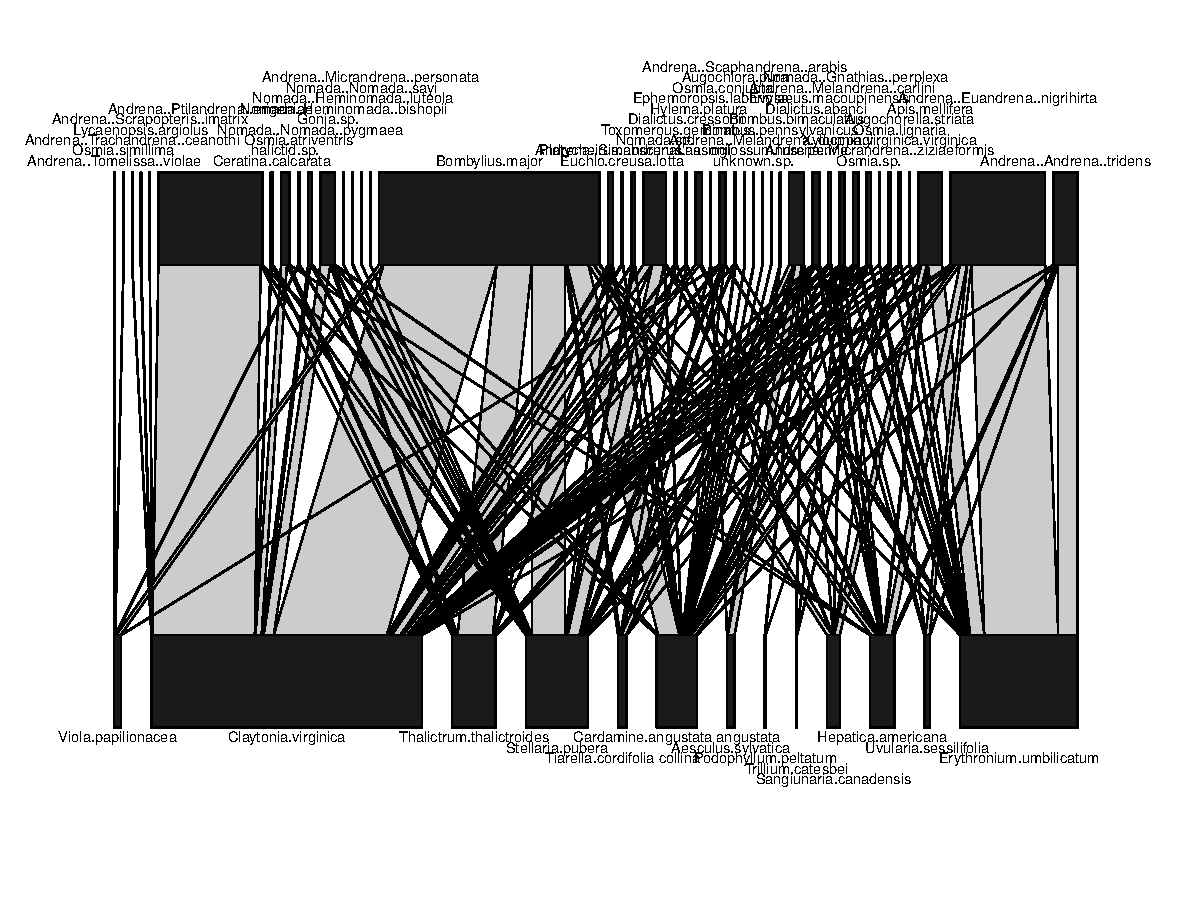
\includegraphics[width=0.8\textwidth]{figures/motten1982_plotweb}
	\smallskip
	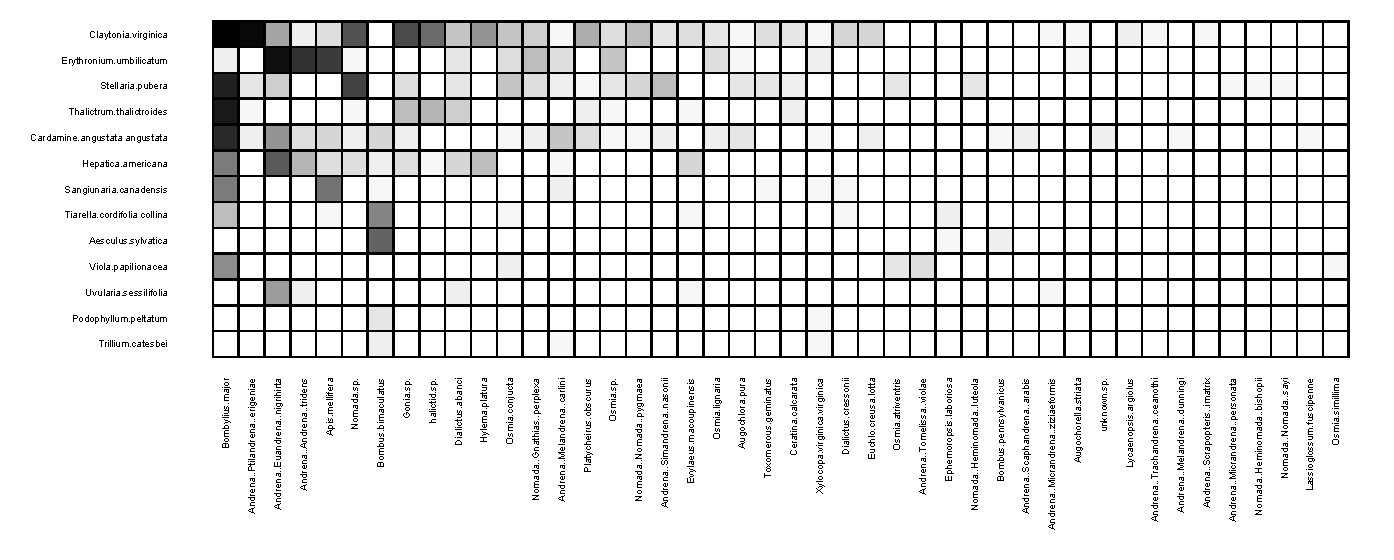
\includegraphics[width=0.8\textwidth]{figures/motten1982_visweb}
	\caption{A bipartite graph of Motten's (1982) pollination network (\emph{top}) and a visualisation of the adjacency matrix (\emph{bottom}). The darker a cell is represented, the more interactions have been observed. By default, \texttt{plotweb} minimises overlap of lines and \texttt{visweb} sorts by marginal totals.}
	\label{fig:Amotten}
\end{figure}



The function \indR{plotPAC} visualises  (Fig.~\ref{fig:AplotPAC}) a very special idea: the potential for apparent competition \citep{Morris2005}. The idea is that every parasitoid emerging from a host can attack another species. Thus, the more individuals emerge from a host, the larger is the potential for these to reduce the competition between hosts, as long as they choose their prey equiprobable. Pretty as it may be, its current value is highest for host-parasitoid networks, so the plot employing a pollination network is for illustration only.
\begin{Schunk}
\begin{Sinput}
plotPAC(PAC(motten1982), outby=0.9)
\end{Sinput}
\end{Schunk}

\begin{wrapfigure}{o}{0.3\textwidth}
	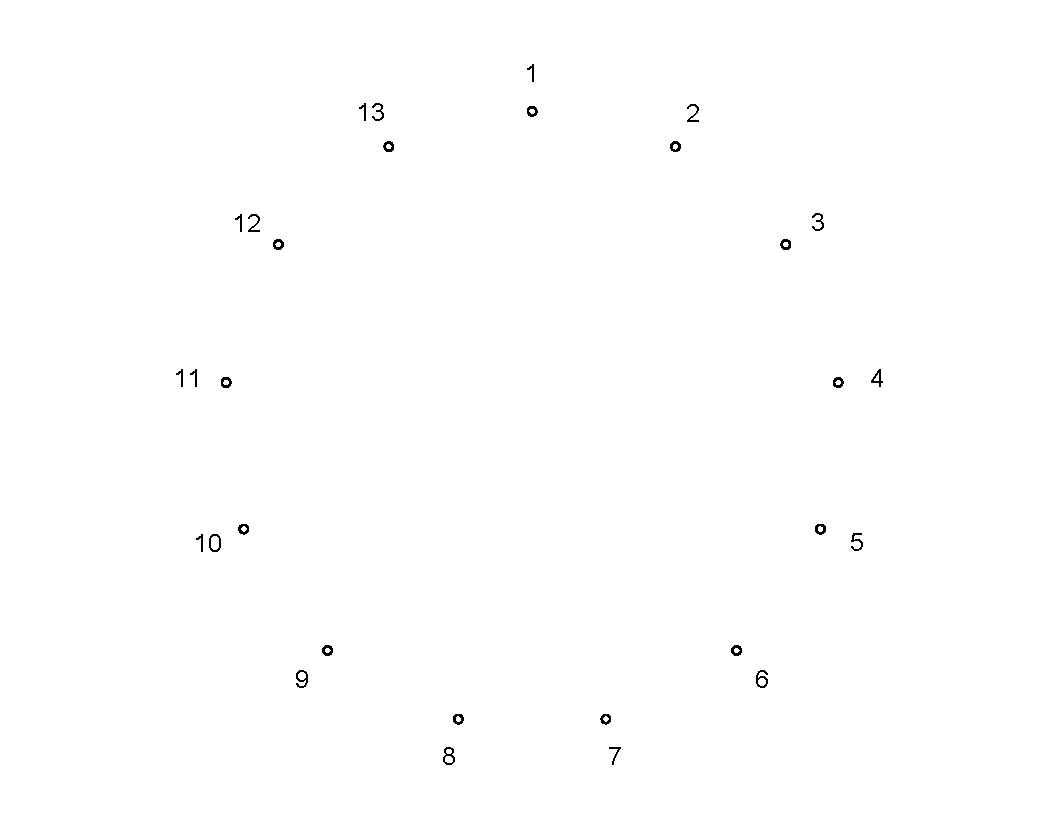
\includegraphics[width=0.3\textwidth]{figures/motten1982_PACplot}
	\caption{A PAC-plot of Motten's \citeyear{Motten1982} pollination network. Lines connect plants potentially visited next by a pollinator. Line width is proportional to probability, which is very similar in this example. See help of \emph{plotPAC} for details on plotting and meaning.}
	\label{fig:AplotPAC}
\end{wrapfigure}
%
We can also visualise communities within the network by computing its modularity and then plotting the result, using the functions \texttt{computeModules} and \texttt{plotModuleWeb}, respectively (Fig.~\ref{fig:Amoduleplot}).
\begin{Schunk}
\begin{Sinput}
mod <- computeModules(motten1982)
plotModuleWeb(mod)
\end{Sinput}
\end{Schunk}
\begin{figure}[h]
\centering
	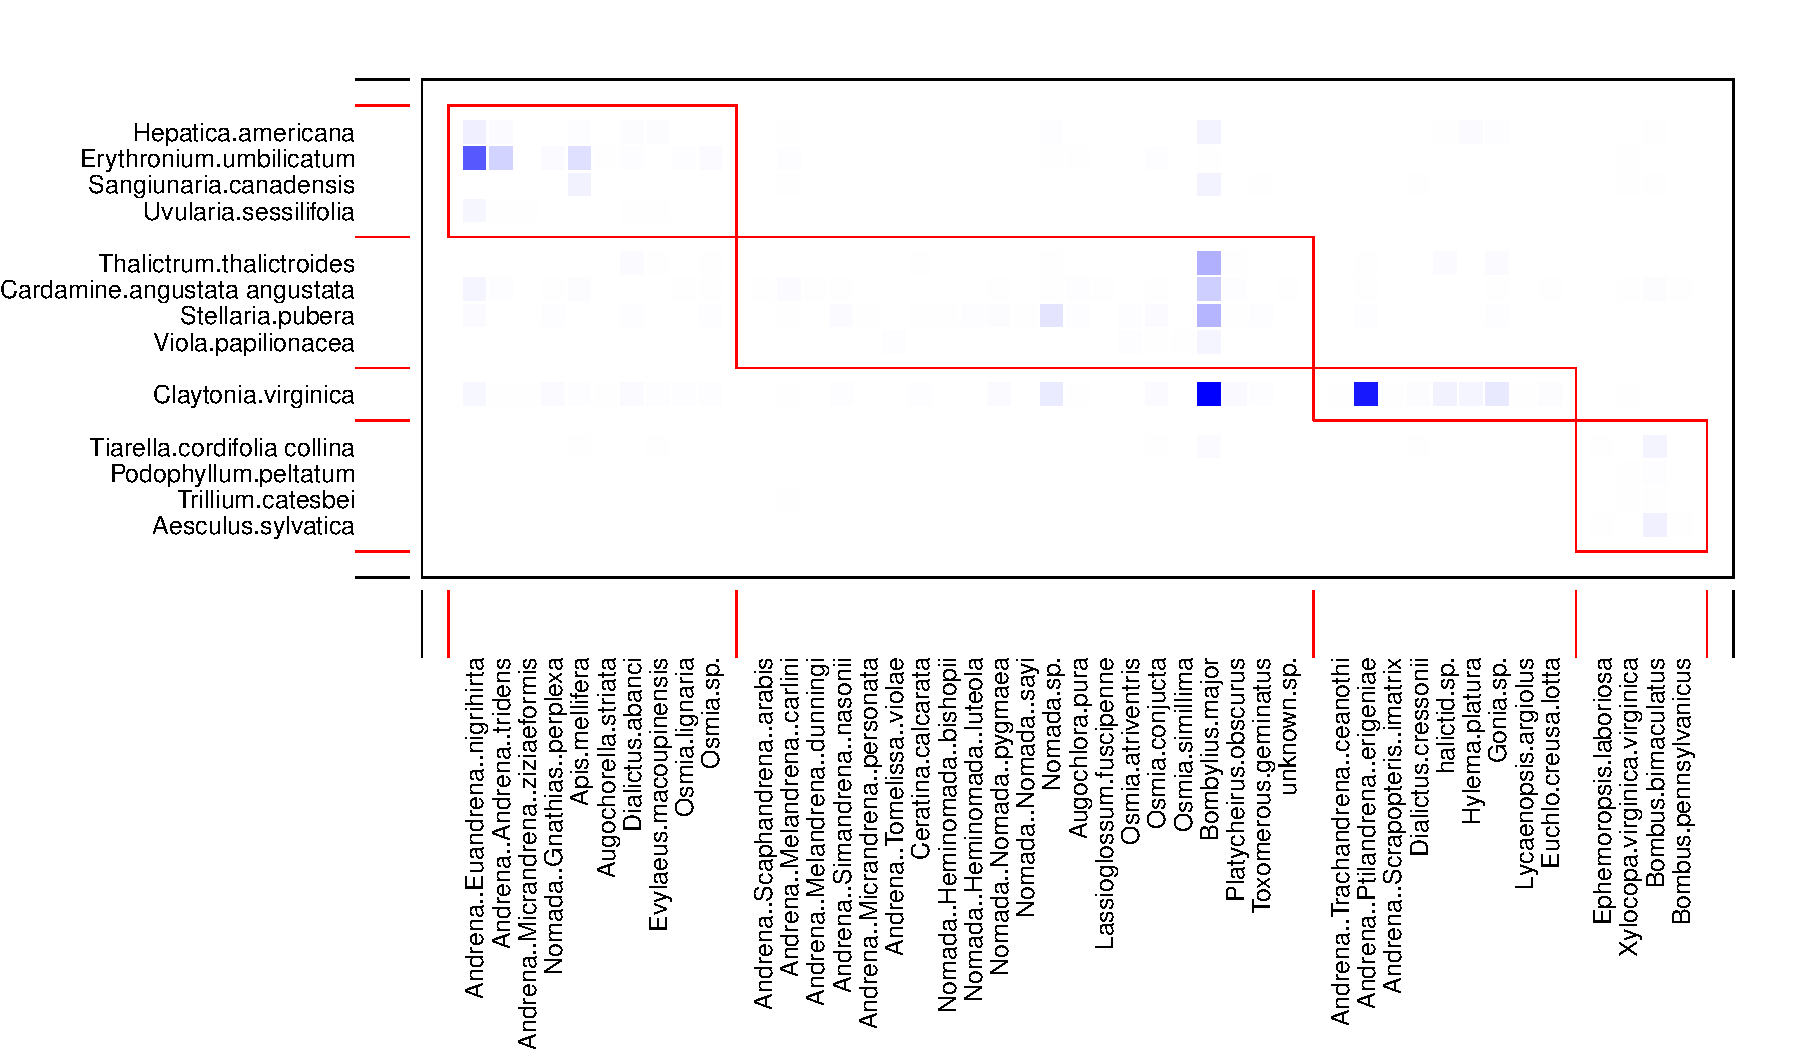
\includegraphics[width=0.7\textwidth]{figures/motten1982_moduleplot}
	\caption{The adjacency matrix of Motten's (1982) pollination network, organised into modules.}
	\label{fig:Amoduleplot}
\end{figure}
%
To visualise either level separately projected into one-mode mode, we have to employ a different package, for example \package{sna} \citep{Butts2013}. We can do the projection on the fly, though. For networks with even a moderate number o species, such plots can become rather obtuse and uninformative (Fig.~\ref{fig:Amottengplot} top).
\begin{Schunk}
\begin{Sinput}
par(mfrow=c(1,2))
gplot(as.one.mode(motten1982, project="higher"), 
 label=colnames(motten1982), gmode="graph", 
label.cex=0.5, vertex.cex=2)
gplot(as.one.mode(motten1982, project="lower"), 
	label=rownames(motten1982), gmode="graph", 
	label.cex=0.75, vertex.cex=2, vertex.col="green")
\end{Sinput}
\end{Schunk}
\begin{wrapfigure}{o}{1\textwidth}
\centering
	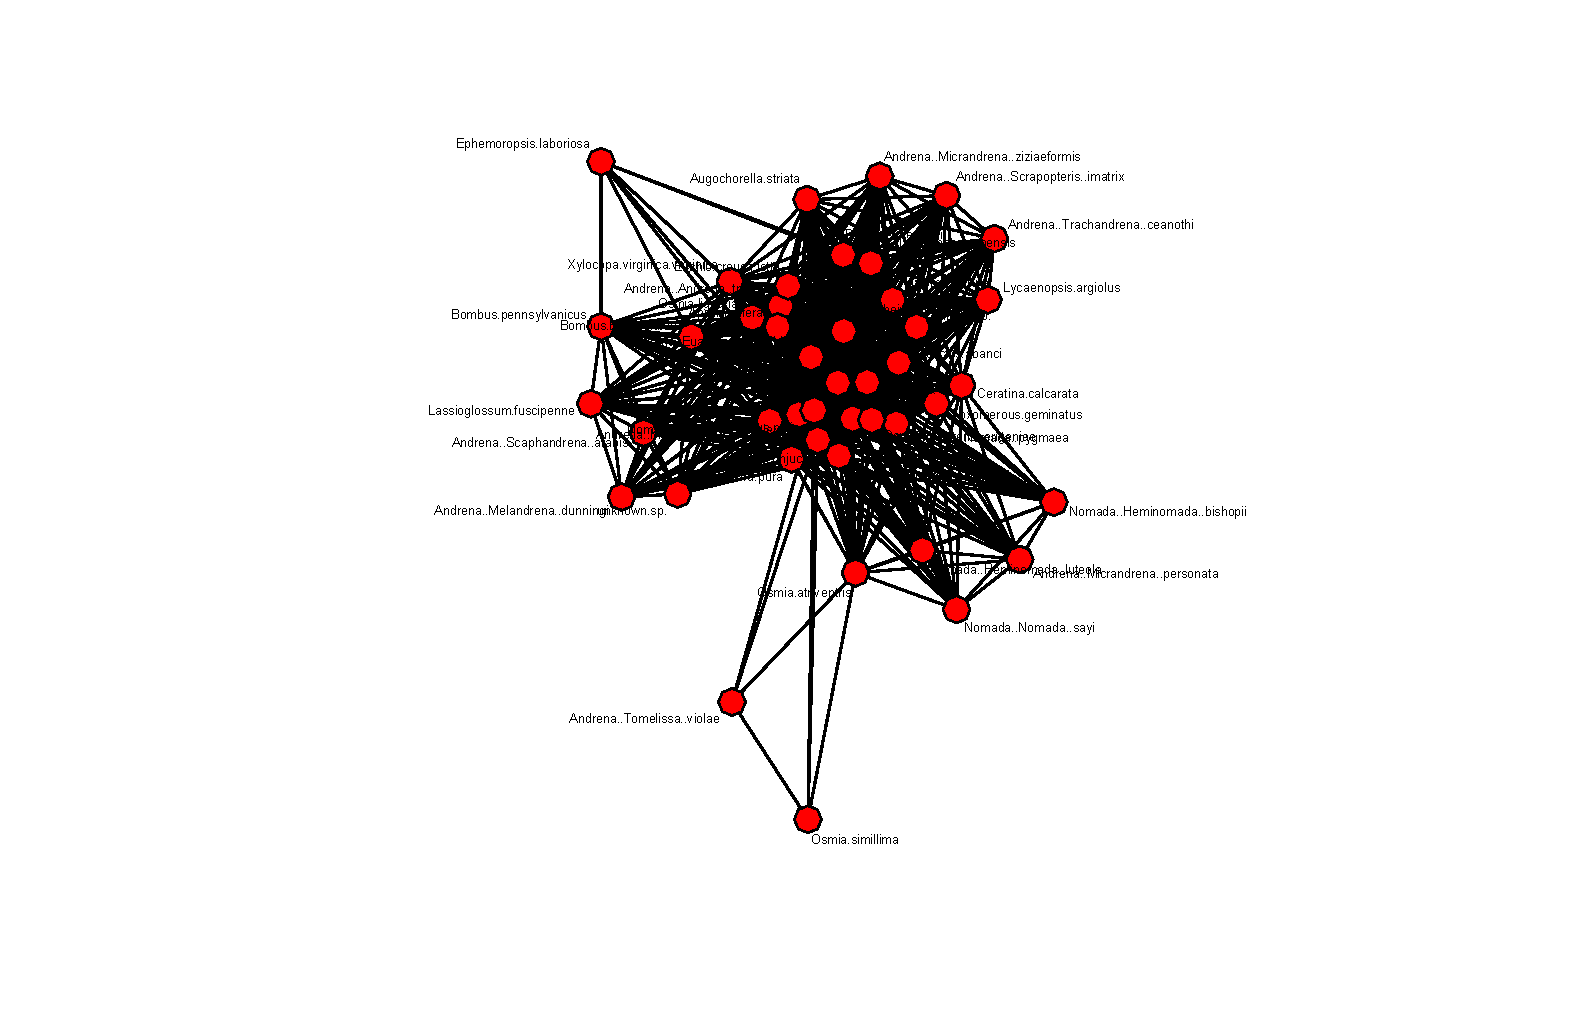
\includegraphics[width=0.45\textwidth]{figures/motten1982_higher_gplot}
	\hfill
	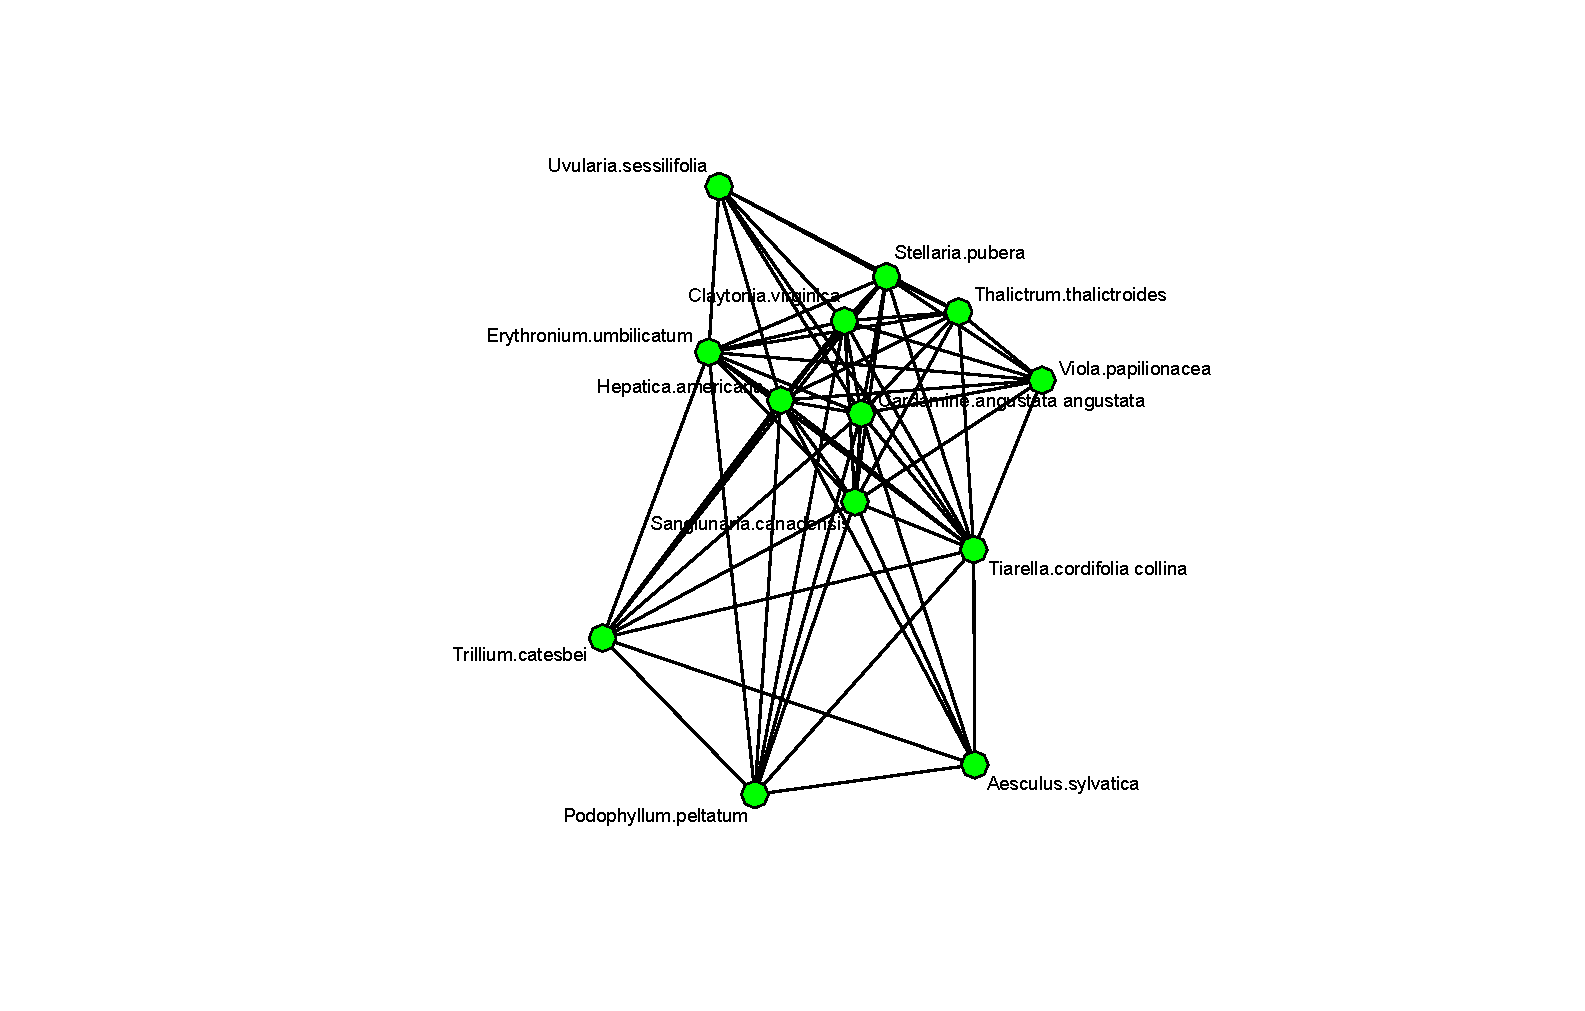
\includegraphics[width=0.45\textwidth]{figures/motten1982_lower_gplot}
	\caption{Plots of one-mode projections of Motten's (1982) pollination network. Pollinators in red (\emph{top}), plants in green (\emph{bottom}). Note that these plots are point symmetrically variable, hence every plot will look somewhat different.}
	\label{fig:Amottengplot}
\end{wrapfigure}


\clearpage

\section{Computing indices} %--------------------------------------------------------------------
Network indices are primarily that: metrics to quantify an aspect of the network. Each may have a justification, a purpose, but the information in a matrix is only finite. As a consequence, network indices are highly correlated. There is thus no point in computing all indices in the book; rather should we consider very carefully what we want to test with the data and select one (or a few) indices to do so.

The \package{bipartite}-package offers itself to data dredging: with one function one can compute dozens of indices, certainly some of them will be significantly correlated with whatever we want to test. While analyses are commonly carried out in this way, this is obviously statistically inappropriate. Two issues are important here. One is that of multiple testing, and there are dozens of publications covering this issue. The other is an attempt to formalise one's expectation. Null models are a way to do so, in particular one's expectation of what a pattern is like in the absence of a process. This technical details of this topic are covered further below (section \ref{sec:A:nullmodels}). 

Indices (currently) come at the following hierarchical levels:
\begin{enumerate}
\item network-level (a single value, per index, for the entire network);
\item group-level  (a value, per index, for each of the two groups);
\item link-level  (a value, per index, for each edge = link);
\item node-level (a value, per index, for each node = species); and
\item species-level (a value, per index, for each species).
\end{enumerate}



\subsection{Network-level indices}\label{networklevel}
This set of indices is computed for the entire network. They are called using the function \indR{networklevel}, which additionally (and conveniently) makes available all indices from the group level, too. Those restricted to the network-level are:
\begin{enumerate}
\item \texttt{\ind{connectance}}, also called `standardised number of species combinations' in biogeographic analyses \citep{Gotelli1996, Dunne2002};
\item \texttt{web asymmetry}, the balance of the number of species in the two levels \citep{Bluethgen2007}; 
\item \texttt{links per species};
\item \texttt{number of compartments};
\item \texttt{compartment diversity} \citep{Tylianakis2007};
\item \texttt{cluster coefficient}, which will compute both the network-wide binary, one-mode-based cluster coefficient as well as those for each level,
\item \texttt{nestedness}, with the returned value indicating the `temperature' of the matrix, which is low ($0$) for a perfectly nested matrix \citep{RodriguezGirones2006};
\item \texttt{weighted nestedness}, or more specifically `weighted interaction nestedness estimator' (WINE), with $1$ indicating perfected nestedness (thus exactly opposite to the previous index) \citep{Galeano2009a};
\item \texttt{weighted NODF}, as an alternative measure of quantitative nestedness, automatically correcting for matrix filling and also indicating nestedness by values towards $1$ \citep{AlmeidaNeto2011}; 
\item \texttt{interaction strength asymmetry} \citep{Bluethgen2007} \citep[or alternatively \texttt{ISA} or \texttt{dependence asymmetry}][]{Bascompte2003}, which quantify whether specialised species interacts with generalised ones in the other level (or vice versa);
\item \texttt{specialisation asymmetry} (or alternatively \texttt{SA}), following the same idea as the previous, but this being based on species specialisation in $d'$;
\item \texttt{linkage density}, marginal totals-weighted diversity of interactions per species \citep{Bersier2002};
\item \texttt{Fisher alpha}, diversity index based on fitting a Fisher-series \citep{Fisher1943};
\item \texttt{interaction evenness}  quantifies how balanced the distribution of interactions is across species, based on Shannon's diversity \citep{Tylianakis2007};
\item \indR{Alatalo interaction evenness}, as an alternative measure of interaction evenness, attempting to overcome some of the shortcomings of the previous, Shannon's, version \citep{Alatalo1981,Muller1999};
\item \texttt{Shannon diversity};
\item \texttt{H2}, network-wide specialisation index $H_2'$ \citep{Bluethgen2006}.
\end{enumerate}

\noindent Similarly to the previous sets of indices, several options are available to fine-tune those in \texttt{networklevel}:
\begin{Schunk}
\begin{Sinput}
networklevel(bezerra2009, index=c("ISA", "weighted NODF", "Fisher alpha"), SAmethod="log")
\end{Sinput}
\begin{Soutput}
                 weighted NODF interaction strength asymmetry 
                  5.717160e+01                   8.842823e-05 
                  Fisher alpha 
                  8.793400e+00 
\end{Soutput}
\end{Schunk}





\subsection{Group-level indices}\label{grouplevel}
Indices that can be computed for each group separately are collected in the function \indR{grouplevel}.\footnote{If network-level indices are also desired, all indices in \texttt{grouplevel} are also accessible through \texttt{networklevel}, see below.} Quite a few of these indices are aggregates from the species level (e.g. by averaging species' degrees), in which case the mean is weighted by the number of observations of each species, thus giving more weight to species for which information is more reliable.\footnote{The weighting can be switched off by stating \texttt{weighted=FALSE}.} Others are biogeographic indices which change their value when the matrix is inverted (i.e. when a group changes from ``species'' to ``islands''). The following indices are implemented:
\begin{enumerate}
\item \texttt{number of species} in the respective trophic level;
\item \texttt{mean number of links};
\item \texttt{mean number of shared partners} \citep{Roberts1990,Stone1992}; 
\item \texttt{cluster coefficient}, which supposedly informs us whether a network has `small world' properties \citep{Watts1998};
\item \texttt{weighted cluster coefficient}, which takes into account the number of interactions and is a properly derived bipartite version of the previous one-mode cluster coefficent above \citep{Opsahl2010};
\item \texttt{togetherness} as the mean number of co-occurrences across all pairwise species combinations \citep{Stone1992};
\item \texttt{\ind{C score}}, or `checkerboardness', which averages the number of instances of 01/10-patterns (i.e. exclusive occurrences) for all pairwise species combinations \citep{Stone1990};
\item \texttt{\ind{V ratio}}, the variance ratio of species numbers to interaction numbers within species of a level \citep{Schluter1984};
\item \texttt{\ind{discrepancy}}, the number of links one would have to move to achieve perfect nestedness \citep{Brualdi1999};
\item \texttt{degree distribution}, fitting an exponential function and (truncated) power laws\citep{Jordano2003};
\item \texttt{extinction slope}, with different options for the extinction sequence \citep{Memmott2004};
\item \texttt{robustness}, the area under the extinction curve \citep{Burgos2007};
\item \texttt{niche overlap}, with options for distance metrics \citep{Pielou1972,Hurlbert1978};
\item \texttt{\ind{generality}} (for the higher trophic level) or \texttt{\ind{vulnerability}} (for the lower one) \citep{Bersier2002};
\item \texttt{partner diversity}, simply the mean Shannon diversity of interactions of each species in a level;
\item \texttt{effective partners} as before, but as the exponent of the base to which Shannon was computed (typically $e$ or $2$) \citep{Jost2006};
\item \texttt{fd} (or alternatively \texttt{\ind{functional diversity}}), which is similar to niche overlap but computed as branch length of a cluster diagram of dissimilarity of resource use \citep{Devoto2012}.
\end{enumerate}

\noindent As in the case of species-level indices, some allow for normalisation (between 0 and 1), others for different basis to the logarithm or similar tuning. A typical call to \texttt{grouplevel} will thus comprise the list of desired indices\footnote{Or alternatively the argument \texttt{index="ALL"}.} and their options, as well as the level(s) for which the computation shall be carried out:
\begin{Schunk}
\begin{Sinput}
grouplevel(bezerra2009, level="both", index=c("mean number of links", "weighted 
     cluster coefficient", "effective partners", "niche overlap"), dist="bray")
\end{Sinput}
\begin{Soutput}
mean.number.of.links.HL mean.number.of.links.LL        niche.overlap.HL 
              9.9502551               7.0975057               0.2824538 
       niche.overlap.LL           generality.HL        vulnerability.LL 
              0.4795595               8.0590841               5.6963672 
\end{Soutput}
\end{Schunk}
The LL and HL behind each index indicate that it was computed for the lower and higher level, respectively. A relatively comprehensive comparison of network-level indices \citep{Dormann2009}, including some at the group level, has shown substantial redundancy among these indices, and few of them have a sound theoretical basis.



\subsection{Node-level indices}\label{nodelevel}
...



\subsection{Link-level indices}\label{linklevel}
At the moment, only few indices have been investigated at the level of the individual link (i.e. the cell of a network matrix):
\begin{enumerate}
\item dependence \citep[i.e. the relevance of each species for the other level][]{Bascompte2006} one matrix for each level;
\item endpoint degree \citep[i.e. product of degrees of species linked by this cell][]{Barrat2004}.
\end{enumerate}
It is employed by simply applying it to the network under consideration and selecting the index desired:
\begin{Schunk}
\begin{Sinput}
str(linklevel(bezerra2009, index=c("dependence", "endpoint")))
\end{Sinput}
\begin{Soutput}
List of 3
 $ HL dependence: num [1:13, 1:13] 0.193 0.131 0.056 0.108 0.105 ...
  ..- attr(*, "dimnames")=List of 2
  .. ..$ : chr [1:13] "Diplopterys.pubipetala" "Byrsonima.gardnerana" "Banisteriopsis.muricata" "Heteropterys.sp1" ...
  .. ..$ : chr [1:13] "Centris.aenea" "Centris.fuscata" "Centris.caxiensis" "Centris.tarsata" ...
 $ LL dependence: num [1:13, 1:13] 0.2415 0.2238 0.0997 0.2474 0.2632 ...
  ..- attr(*, "dimnames")=List of 2
  .. ..$ : chr [1:13] "Diplopterys.pubipetala" "Byrsonima.gardnerana" "Banisteriopsis.muricata" "Heteropterys.sp1" ...
  .. ..$ : chr [1:13] "Centris.aenea" "Centris.fuscata" "Centris.caxiensis" "Centris.tarsata" ...
 $ endpoint     : num [1:13, 1:13] 117 78 156 104 91 65 52 26 52 52 ...
  ..- attr(*, "dimnames")=List of 2
  .. ..$ : chr [1:13] "Diplopterys.pubipetala" "Byrsonima.gardnerana" "Banisteriopsis.muricata" "Heteropterys.sp1" ...
  .. ..$ : chr [1:13] "Centris.aenea" "Centris.fuscata" "Centris.caxiensis" "Centris.tarsata" ...
\end{Soutput}
\end{Schunk}
This function is so rudimentary, and its output so disproportionally voluminous, that it is not worth going into further details here and use \texttt{str} to only show the structure of the output.




\subsection{Species-level indices}\label{specieslevel}
The (growing) list of indices computable for each species in the network comprises (the index name to be used in the call is given in \texttt{typewriter} font):
\begin{enumerate}
\item \texttt{degree}, i.e. the number of links of each species,
\item \texttt{normalised degree} for a normalised version of degree \citep{MartinGonzalez2010},
\item \texttt{species strength} as sum of dependencies for each species \citep{Bascompte2006},
\item \indR{nestedrank} as rank in a nested matrix \citep{Alarcon2008},
\item \texttt{interaction} for interaction push/pull (a version of dependence asymmetry), \citep{Vazquez2007},
\item \texttt{PDI} for \ind{Paired Differences Index} \citep{Poisot2011,Poisot2011a},
\item \indR{resource range} for Schoener's index of unused resources \citep{Schoener1989},
\item \texttt{species specificity} (or coefficient of variation of interactions) \citep{Julliard2006,Poisot2012a},
\item \texttt{PSI} for \ind{pollination service index} (or pollinator support index, depending on the trophic level),\footnote{devised by the author with Nico Blüthgen and Bernd Gruber}
\item \texttt{NS} for \ind{node specialisation index} \citep{Dalsgaard2008},
\item \indR{betweenness} for betweenness \citep{Borgatti1997},
\item \indR{closeness} (both automatically also return their weighted counterparts proposed by Tore Opsahl in package \package{tnet}),
\item \texttt{Fisher} for \ind{Fisher's alpha} as a measure of diversity \citep{Fisher1943},
\item \texttt{diversity} for Shannon diversity of interactions of that species,
\item \texttt{effective partners} for the effective number of interacting partners \citep{Bersier2002},
\item \texttt{proportional generality} for a quantitative version of normalised degree,\footnote{devised by Jochen Fründ}
\item \texttt{proportional similarity} as specialisation measured as similarity between use and availability \citep{Feinsinger1981},
\item \texttt{d} for Blüthgen's $d'$ \citep{Bluethgen2006}.
\end{enumerate}

\noindent Some of them allow for normalisation (between 0 and 1), others for different basis to the logarithm or similar tuning. A typical call to \texttt{specieslevel} will thus comprise the list of desired indices\footnote{Or alternatively the argument \texttt{index="ALL"}.} and their options, as well as the level(s) for which the computation shall be carried out:
\begin{Schunk}
\begin{Sinput}
specieslevel(bezerra2009, level="lower", index=c("normalised degree", "PDI", 
      "effective partners"), PDI.normalise=F)
\end{Sinput}
\begin{Soutput}
                           normalised.degree       PDI effective.partners
Diplopterys.pubipetala             0.6923077 1010.0000           7.437631
Byrsonima.gardnerana               0.4615385 1939.6667           3.819660
Banisteriopsis.muricata            0.9230769  657.0000           9.191488
Heteropterys.sp1                   0.6153846  570.3333           6.278285
Heteropterys.sp2                   0.5384615  567.3333           5.865968
Dicella.bracteosa                  0.3846154  429.0000           4.582040
Carolus.chasei                     0.3076923  513.6667           3.751208
Stigmaphyllon.paralias             0.1538462  774.0000           1.944388
Banisteriopsis.stellaris           0.3076923  245.6667           3.787887
Banisteriopsis.schizoptera         0.3076923  189.0000           3.822392
Stigmaphyllon.auriculatum          0.3076923  204.3333           3.687447
Stigmaphyllon.ciliatum             0.2307692  238.0000           2.937197
Janusia.anisandra                  0.2307692  220.3333           2.813322
\end{Soutput}
\end{Schunk}
A relatively comprehensive comparison of species-level indices of specialisation \citep{Dormann2011} has shown substantial redundancy among these indices, and few of them have a sound theoretical basis \cite{Poisot2012a}.



\subsection{Which index to chooose?}%--------------------------------------------------------------
Different indices were invented (``developed'') for different purposes. However, for most indices, it has not been demonstrated that they actually achieve what their inventor had in mind. Most commonly indices quantify a specific pattern which may have come about by a whole variety of different causes. Take, for example, connectance, i.e. the proportion of possible links actually recorded. Low connectance may be caused by high specialisation or by low samplng intensity. The same holds true for a species' degree, which (typically) increases with sampling effort as well as generalisation. For the choice of an index this means that we cannot solely rely on what the inventor has proposed this index to be good for, but we have to keep in mind that it may actually quantify several other things, too.

Apart from the different levels at which an index can quantify a network pattern (from the individual link to the entire network, as covered in sections \ref{linklevel}--\ref{networklevel}), indices can be divided into those for binary and those for weighted data (called here binary and weighted indices, respectively). Binary indices only use the information of whether a link exists, while weighted indices additionally account for how strong a link is, as judged from the actual value in a network matrix.%\footnote{This is the difference between graph $\vec{A}$ and graph $\vec{B}$ in section \ref{sec:graphtheory}.}

Binary indices, by definition, use less information. It does not follow that they are thus more robust! In fact, \citet{Bluethgen2010} argues the opposite, since only a weighted index can tell whether an observed value indicates specialisation or not.\footnote{Imagine two species, one with entries (1, 1), the other with entries (1, 100). A binary index would not be able to tell between them, while a quantitative would expose the second as far more specialised.} 

This, if two indices are available to quantify the same idea, one binary and one quantitative, one should generally choose the quantitative one. Rather than species degree, we should use species strength or linkage density. Table \ref{tab:binaryquantitative} depicts some such binary-quantitative index pairs.
%
\begin{table}
\label{tab:binaryquantitative}
\caption{Binary-quantitative pairs of network indices. Note: Most quantitative indices can also be computed on binary networks. That does not make them a quantitative measure!}
\begin{tabular}{l|ll}
\hline
& binary & quantitative \\ \hline
%link level    & --     & --           \\ \hline
network level & connectance & $H_2'$\\ 
& links per species & linkage density \\ 
& nestedness        & weighted NODF, wine \\ %\hline
group level   & mean number of partners & effective number of partners \\%\hline
species level & degree & species strength, effective number of partners \\\hline
\end{tabular}
\end{table}


In a nutshell: Quantitative indices make use of more information in the data. They are generally more advisable, although most of them also are strongly affected by sampling issues.


\bigskip

The Rnw source of this document is at \url{https://github.com/biometry/bipartite/bipartite/vignettes/Intro2bipartite.Rnw}.

%\backmatter % only if document type is book!
%\begin{fullwidth}
\setlength{\bibsep}{0cm}
\def\bibfont{\small}

\bibliographystyle{mee} %all show doi, url, isbn; haven't found out yet how to switch that off
\bibliography{bipartite}
%\end{fullwidth}

\printindex



\end{document}
